%% Source of figures/harness-architecture.pdf (rules/04-figures-tables.md).
%% Build: xelatex -output-directory=figures figures/src/harness-architecture.tex
%% Drawn from OpenTrading 7319264: src/core/runtime.ts, agent.ts, tools/wrap.ts, providers.ts, session/store.ts.
\documentclass[border=2pt]{standalone}
\usepackage{fontspec}
\IfFontExistsTF{Arial}{\setmainfont{Arial}}{\setmainfont{TeX Gyre Heros}}
\usepackage{tikz}
\usetikzlibrary{positioning,arrows.meta,fit,backgrounds,calc}
\begin{document}
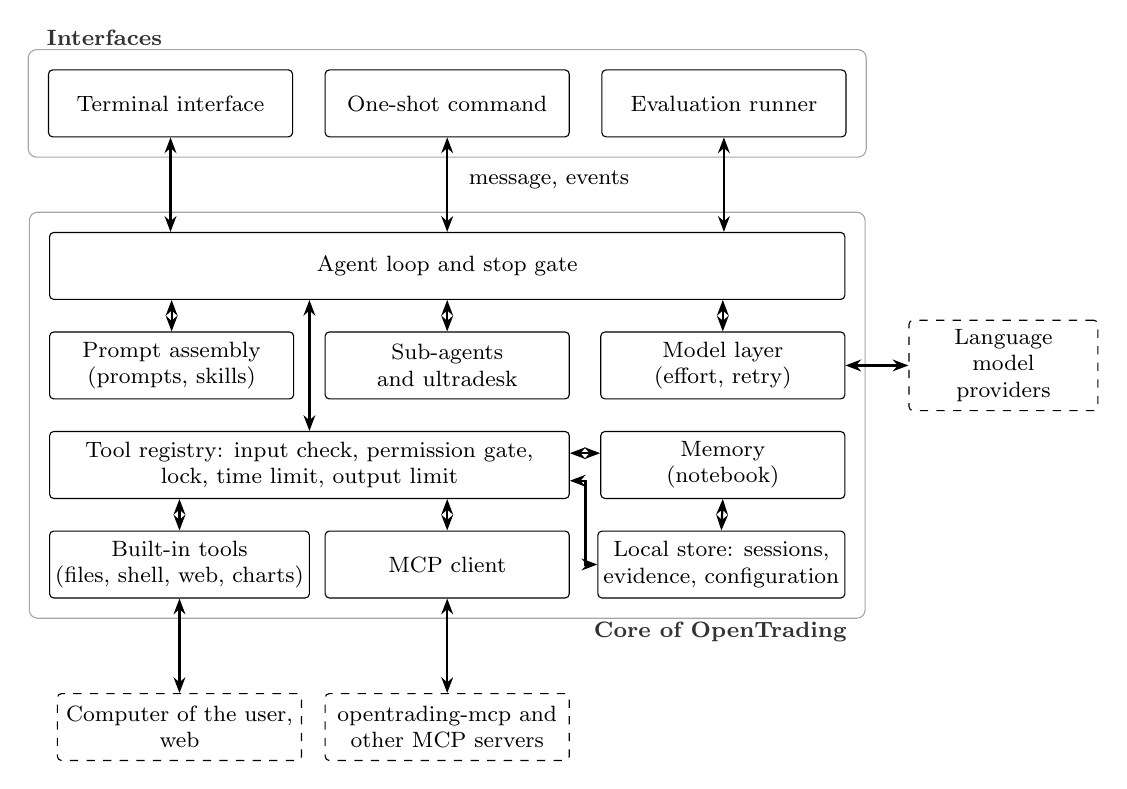
\begin{tikzpicture}[
  font=\fontsize{8}{9.5}\selectfont,
  box/.style={draw, rounded corners=1.5pt, align=center, minimum height=8.5mm, inner xsep=2pt, fill=white},
  ext/.style={box, dashed},
  arr/.style={-{Stealth[length=2mm]}, thick},
  both/.style={{Stealth[length=2mm]}-{Stealth[length=2mm]}, thick},
  group/.style={draw, gray!70, rounded corners=3pt, inner xsep=2.5mm, inner ysep=2.5mm},
  glabel/.style={font=\fontsize{8}{9.5}\selectfont\bfseries, anchor=south west, gray!40!black, inner sep=1pt}
]
\node[box, minimum width=31mm] (tui) {Terminal interface};
\node[box, minimum width=31mm, right=4mm of tui] (print) {One-shot command};
\node[box, minimum width=31mm, right=4mm of print] (eval) {Evaluation runner};

\node[box, minimum width=101mm, below=12mm of print] (loop) {Agent loop and stop gate};
\node[box, minimum width=31mm, below=4mm of loop.south west, anchor=north west] (prompt) {Prompt assembly\\(prompts, skills)};
\node[box, minimum width=31mm, below=4mm of loop.south] (sub) {Sub-agents\\and ultradesk};
\node[box, minimum width=31mm, below=4mm of loop.south east, anchor=north east] (model) {Model layer\\(effort, retry)};
\node[box, minimum width=66mm, below=4mm of prompt.south west, anchor=north west] (reg) {Tool registry: input check, permission gate,\\lock, time limit, output limit};
\node[box, minimum width=31mm, below=4mm of model.south east, anchor=north east] (mem) {Memory\\(notebook)};
\node[box, minimum width=31mm, below=4mm of reg.south west, anchor=north west] (local) {Built-in tools\\(files, shell, web, charts)};
\node[box, minimum width=31mm, below=4mm of reg.south east, anchor=north east] (mcp) {MCP client};
\node[box, minimum width=31mm, below=4mm of mem.south east, anchor=north east] (store) {Local store: sessions,\\evidence, configuration};

\node[ext, minimum width=31mm, below=12mm of local] (os) {Computer of the user,\\web};
\node[ext, minimum width=31mm, below=12mm of mcp] (srv) {opentrading-mcp and\\other MCP servers};
\node[ext, minimum width=24mm, right=8mm of model] (llm) {Language\\model\\providers};

\draw[both] (tui.south) -- (tui.south |- loop.north);
\draw[both] (print.south) -- (loop.north);
\draw[both] (eval.south) -- (eval.south |- loop.north);
\draw[both] (prompt.north) -- (prompt.north |- loop.south);
\draw[both] (sub.north) -- (loop.south);
\draw[both] (model.north) -- (model.north |- loop.south);
\coordinate (gap) at ($(prompt.east)!0.5!(sub.west)$);
\draw[both] (gap |- reg.north) -- (gap |- loop.south);
\draw[both] (local.north) -- (local.north |- reg.south);
\draw[both] (mcp.north) -- (mcp.north |- reg.south);
\draw[both] (local.south) -- (os.north);
\draw[both] (mcp.south) -- (srv.north);
\draw[both] (model.east) -- (llm.west);
\draw[both] (mem.south) -- (store.north);
\draw[both] ([yshift=1.5mm]reg.east) -- ([yshift=1.5mm]mem.west);
\draw[both] ([yshift=-2mm]reg.east) -- ++(2mm,0) |- (store.west);

\begin{scope}[on background layer]
  \node[group, fit=(tui)(eval)] (gi) {};
  \node[glabel] at ([xshift=2mm]gi.north west) {Interfaces};
  \node[group, fit=(loop)(store)(local)] (gc) {};
  \node[glabel, anchor=north east] at ([xshift=-2mm]gc.south east) {Core of OpenTrading};
\end{scope}
\node[anchor=west, align=left] at ([xshift=1.5mm]$(print.south)!0.45!(print.south |- loop.north)$) {message, events};
\end{tikzpicture}
\end{document}
